%%%%%
%%Title: HiPi+Bus V0.2 Chapter 6
%%Creator: Ando Ki
%%CreationDate: April 1992
%%FileName: sec2
%%RelatedFile: ch6
%%%%%
\section{버스클럭의 시간규격}
%
버스 클럭 신호는 본 시스템 버스의 모든 부분의 제어에 있어서 기준이 되는 신호이다.
클럭은 슬롯 10에서 공급되고 다른 슬롯에 위치한 모든 보드들은 이 신호를 받아서 제어 정보로 사용한다.
%
%\documentstyle[a4]{hbook}
%\begin{document}
%
\begin{table}[htbp]
\caption{버스클럭의 시간규격 요약}\label{table:bclk-time}
   \begin{center}
   \begin{tabular}{|l|l|r|r|r|} \hline
	timing parameter & name & min & typical & max \\ \hline \hline
	$TP^{BCLK}_0$ & BCLK* cycle time & 59 & 60 & 61 \\ \hline
	$TP^{BCLK}_1$ & BCLK* high pulse width & - & 30 & - \\ \hline
	$TP^{BCLK}_2$ & BCLK* low pulse width & - & 30 & - \\ \hline
	$TP^{BCLK}_3$ & BCLK* falling transition time & 3 & - & 5 \\ \hline
   \end{tabular}
   \end{center}
\end{table}
%
%\end{document}

\begin{figure}[htb]
    \centerline{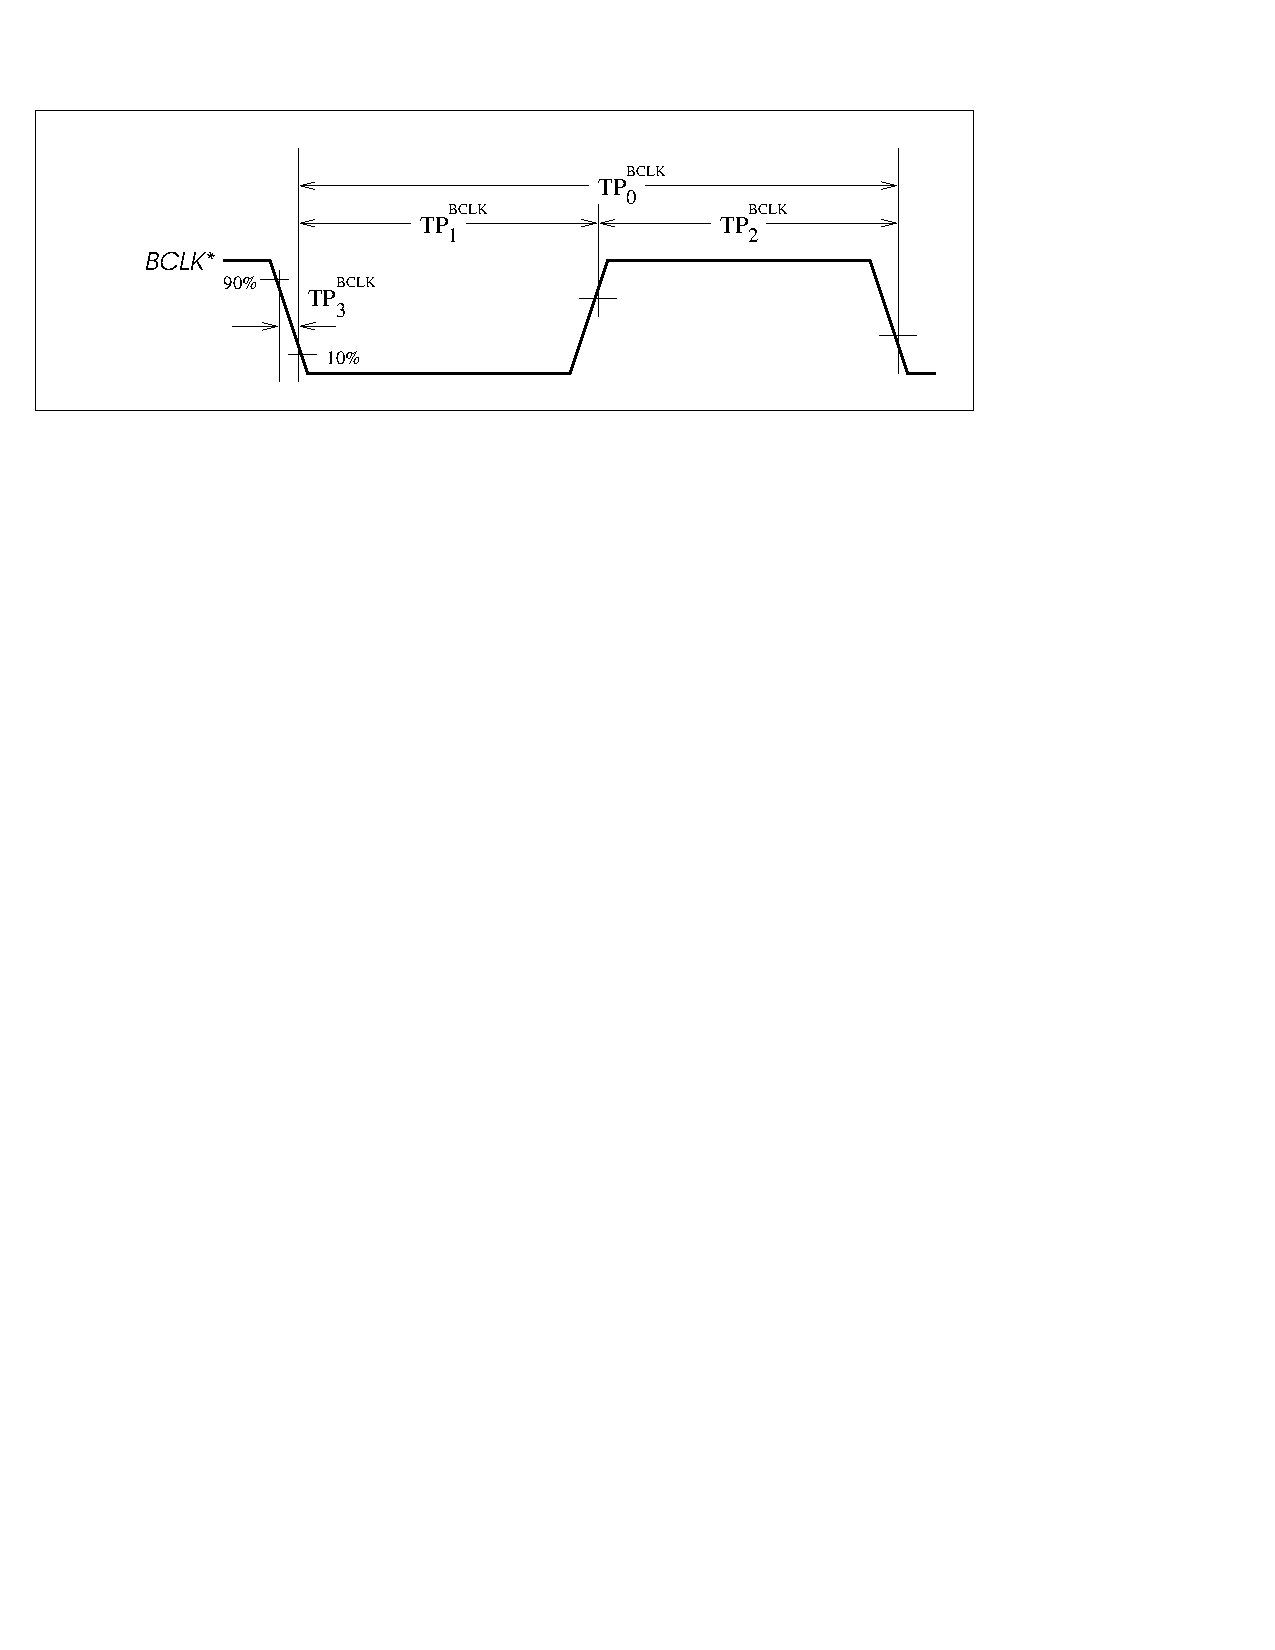
\includegraphics{ch6/FIG/bclk-time.jpg}}
   \caption{버스클럭의 시간규격}\label{figure:bclk-time}
\end{figure}
%

버스클럭의 속도(clock frequency)는 16.5 MHz로
60.6 $n$sec의 주기(clock period, clock cycle time))를
갖으며 정확한 제어를 위하여 
백플레인에 나타나는 버스클럭 신호의 하강점(falling edge)만을
사용하도록 규정하고 시간적 허용오차는 $\pm1 n$sec 이내로 규정한다.
클럭의 Duty Cycle은 50\% ($TP^{BCLK}_1 \div TP^{BCLK}_0$)로 규정한다.
버스클럭 신호가 90\%에서 10\%로 
천이하는 시간인 하강점 천이시간(falling transition time)를
3 $n$sec 이상 5 $n$sec 이내로 규정한다.
%%%%%
